\documentclass[conference]{IEEEtran}
\IEEEoverridecommandlockouts
\usepackage{cite}
\usepackage{amsmath,amssymb,amsfonts}
\usepackage{algorithmic}
\usepackage{graphicx}
\usepackage{textcomp}
\usepackage{xcolor}
\usepackage{tabularx}
\usepackage{multirow}
\usepackage{graphics} % for pdf, bitmapped graphics files
\usepackage{subfig}
\usepackage{subcaption}
\usepackage{hyperref}
\usepackage{academicons}
\usepackage{xcolor}
\usepackage{listings}
\def\BibTeX{{\rm B\kern-.05em{\sc i\kern-.025em b}\kern-.08em
		T\kern-.1667em\lower.7ex\hbox{E}\kern-.125emX}}
% Gráficas en MATLAB
\usepackage{tikz, pgfplots}
% Color Enlace
\definecolor{colorEnlace}{RGB}{0, 0, 0}
\hypersetup{
	colorlinks=true,
	linkcolor=colorEnlace,
	citecolor=colorEnlace,
	urlcolor=colorEnlace,
	pdfauthor={Ruth Juana Espino Puma},
	pdftitle={Controlador }
}
% Control 
\usepackage{amsmath}
\begin{document}
	
	\title{Experiencia N°5 - Diseño de Compensadores}
	
	\author{
		\IEEEauthorblockN{Ruth Juana Espino Puma}
		\IEEEauthorblockA{
			Estudiante de Ingeniería Electrónica \\
			Cusco, Perú \\
			184657@unsaac.edu.pe}
		\and
		\IEEEauthorblockN{Davis Bremdow Salazar Roa}
		\IEEEauthorblockA{
			Estudiante de Ingeniería Electrónica \\
			Cusco, Perú \\
			200353@unsaac.edu.pe
		}
		\and
		\IEEEauthorblockN{Ing. Darcy Arredondo Huarac}
		\IEEEauthorblockA{
			Laboratorio de Control I\\
			Cusco, Perú\\
			diego.arredondo@unsaac.edu.pe}
	}
	\maketitle
	
	\begin{abstract}
		Lead-lag compensators are crucial tools in control system design. They are used to shape the frequency response of a system, improving its stability and performance. By strategically placing a zero and a pole, these compensators can enhance the system's transient response, increasing the speed and reducing overshoot. Additionally, they can help to improve the steady-state error, ensuring that the system reaches its desired output. The design process typically involves analyzing the system's Bode plot to identify the frequency range where compensation is needed, and then selecting the appropriate values for the zero and pole locations to achieve the desired performance. Lead-lag compensators offer a versatile solution for a wide range of control problems and are widely used in industrial applications.
	\end{abstract}
	
	\begin{IEEEkeywords}
		Lead compensator, Lag compensator, lead-lag compensator, phase lead, phase lag,transfer function, pole-zero plot, transient response, steady-state error
	\end{IEEEkeywords}
	\section{Informe Final}
	
	 \subsection{\textbf{Muestre el procedimiento del cálculo de las resistencias y capacitores del diseño del circuito de la Figura 1 para el caso Subamortiguado y Sobreamortiguado en lazo cerrado}}
	 
	 El circuito mostrado en la figura \ref{fig:circuito-adelanto-atraso} nos permite modelar modelar las partes fundamentales para la compensación de las plantas subamortiguadas y/o sobreamortiguadas que son sistemas de segundo orden como se define en \cite{ogata2015} y siendo estas el restador definido por U1 y el compensador en atraso adelanto definido por U2 y U3 las cuales se encargan de modificar el comportamiento de la planta a los valores deseados.
	 
	 \begin{figure}[h]
	 	\centering
	 	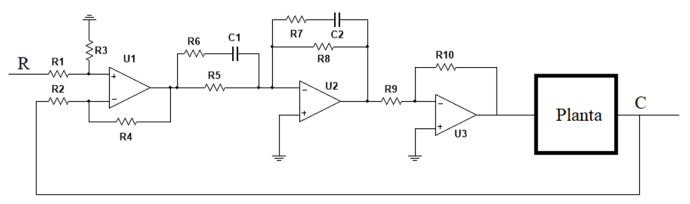
\includegraphics[width=0.5\textwidth]{media/circuito-adelanto-atraso}
	 	\caption{Circuito del compensador adelanto - atraso}
	 	\label{fig:circuito-adelanto-atraso}
	 \end{figure}
	 
	     
	 Para el caso del amplificador operacional configurado como restador, es necesario que todas sus resistencias tenga el mismo valor para que este funcione correctamente por lo tanto los valores de $R_1 = R_2 = R_3 = R_4 = 1K [\Omega]$, para el resto de resistencias fue necesario en concreto para el compensador de atraso adelanto, fue necesario considerar la función de transferencia general la cual se define en \ref{eq:ft-compensador-sub} y los parámetros y valores de la misma que se definen en \ref{eq:parametro-compensador} y \ref{eq:ganancia-compensador}
	 
	 \begin{equation}
	 	\frac{E_o(s)}{E_i(s)} = \frac{R_8 R_{10}}{R_5 R_9} \left[ \frac{(R_5 + R_6)C_1s + 1}{R_6C_1s + 1} \right] \left[ \frac{R_7C_2s + 1}{(R_7 + R_8)C_2s + 1} \right]
	 	\label{eq:ft-compensador-general}
	 \end{equation}
	 
	 Los parámetros para cada compensador teniendo la forma general de los compensadores de atraso y adelanto, se definen en \ref{eq:parametro-compensador}
	 \begin{align}
	 	T_1 = (R_5 + R_6)C_1, \quad \alpha T_1 = R_6C_1, \quad T_2 = R_7C_2, \quad \beta T_2 = (R_7 + R_8)C_2
	 	\label{eq:parametro-compensador}
	 \end{align}
	 
	 La ganancia total del sistema considerando el efecto del compensador de adelanto y atraso se define en \ref{eq:ganancia-compensador} y mediante la cual se podrá ajustar para adecuar el comportamiento del sistema en lazo cerrado a los requisitos de funcionamiento deseados.
	 
	 \begin{equation}
	 	K_c = \frac{R_7 R_8 R_{10}}{R_5 R_6 R_9} \cdot \frac{R_5 + R_6}{R_7 + R_8}
	 	\label{eq:ganancia-compensador}
	 \end{equation}
	 
	 Finalmente para el cálculo de cada valor resistivo y/o capacitivo de forma general se tuvo en cuenta las siguientes relaciones al comparar la función de transferencia general del compensador definida \ref{eq:ft-compensador-general} con las funciones de transferencia para los compensadores diseñados para cada caso, siendo así que se tienen las siguientes relaciones:
	 
	 \begin{align}
	 	R_6 &= \frac{1}{PoloAdelantoC_1} \\
	 	R_5 &= \frac{1}{CeroAdelantoC_1} - R_6 \\
	 	R_7 &= \frac{1}{CeroRetrasoC_2} \\
	 	R_8 &= \frac{1}{PoloRetrasoC_2} - R_7 \\
	 	R_10 &= \frac{K_cR_5 R_6 R_9 (R_7 + R_8)}{R_7 R_8(R_6 + R_5)} \\
	 \end{align}
	 
	 Estableciendo como punto de partida las capacitancias $C_1 y C_2$, las cuales se eligieron a criterio debido a que estas se encuentran limitadas comercialmente en el mercado y la facilidad que brinda su definición en el calculo de las resistencias en función a los polos, ceros y la ganancia total de los compensadores calculados mediante el LGR.
	 
	 \subsubsection{\textbf{Sistema subamortiguado}}
	 En el caso del sistema subamortiguado el compensador en atraso - adelanto la función de transferencia se define en \ref{eq:ft-compensador-sub}
	 \begin{equation}
	 	G_c(s) = \frac{2.5659(s + 10)(s + 25)}{(s + 43.36)(s + 0.1148)}
	 	\label{eq:ft-compensador-sub}
	 \end{equation}
	 
	 Y cual se usara para poder obtener los valores resistivos mediante comparación y las ecuaciones definidas previamente, siendo así que para el caso subamortiguado con las capacitancias $C_1 = C_2 = 47uF$, se tiene:
	 
	 \begin{align}
	 	R_6 &= \frac{1}{43.36*47*10^{-6}} = 490.69646 [\Omega] \\
	 	R_5 &= \frac{1}{10*47*10^{-6}} - 490.69646 = 1636.93 [\Omega] \\
	 	R_7 &= \frac{1}{25*47*10^{-6}} = 851.0638 [\Omega] \\
	 	R_8 &= \frac{1}{0.1148*47*10^{-6}} - 851.0638 = 184485.136 [\Omega] \\
	 	R_{10} &= 537.4356 [\Omega] \\
	 \end{align}
	 
	 Al redondear los resultados a valores comerciales resistivos, estos incrementaron su valor o disminuyeron el mismo sin la necesidad de alterar en gran manera el comportamiento del sistema, lo cual se podrá verificar en una primera etapa mediante la simulación y en una segunda más concreta mediante la implementación del circuito.
	 
	 \subsubsection{\textbf{Sistema sobreamortiguado}}
	 
	 Para el caso del sistema sobreamortiguado la función del transferencia como se define en \ref{eq:ft-compensador-sobre}
	 
	 \begin{equation}
	 	G_c(s) = \frac{10.8843(s + 41.98)(s + 16.8)}{(s + 117.4)(s + 0.5112)}
	 	\label{eq:ft-compensador-sobre}
	 \end{equation}
	 Al igual que con el sistema subamortiguado el calculo de resistencias, se realizara mediante comparación con las ecuaciones definidas previamente y la asignación de capacitancias $C_1 = 47uF y C_2 = 470uF$ para facilitar el calculo resistivo.
	 \begin{align}
	 	R_6 &= \frac{1}{117.4*47*10^{-6}} = 325.5953 [\Omega] \\
	 	R_5 &= \frac{1}{41.98*47*10^{-6}} - 325.5953 = 1636.93 [\Omega] \\
	 	R_7 &= \frac{1}{16.8*470*10^{-6}} = 126.6464 [\Omega] \\
	 	R_8 &= \frac{1}{0.5112*470*10^{-6}} - 126.6464 = 4035.44197 [\Omega] \\
	 	R_{10} &=  4850.43702 [\Omega] \\
	 \end{align}
	 Y como en el caso previo para el caso sobreamortiguado tampoco se pudo apreciar un cambio notable en la respuesta del sistema en la simulación e implementación al redondear los valores resistivos a los comerciales.
	 
	 \subsection{\textbf{Muestre las gráficas obtenidas en el simulador para el caso Subamortiguado y Sobreamortiguado en lazo cerrado}}.
	 
	 \subsubsection{\textbf{Sistema subamortiguado}}
	 Para la simulación de este tipo de sistema de hizo uso del software de simulación NI - MULTISIN 
	 \begin{figure}[h]
	 	\centering
	 	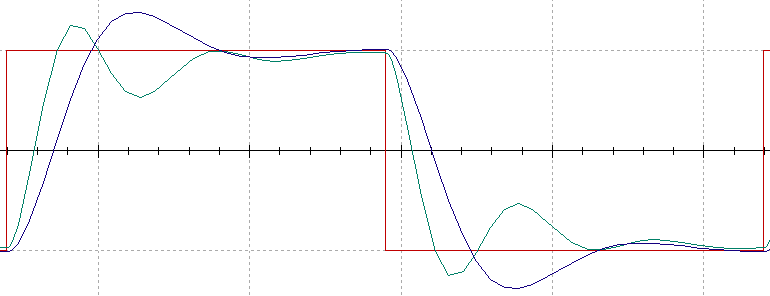
\includegraphics[width=0.5\textwidth]{media/respuesta-sub-multi}
	 	\caption{Respuesta del sistema subamortiguado - MULTISIM}
	 	\label{fig:respuesta-sub-multi}
	 \end{figure}
	 
	 \subsubsection{\textbf{Sistema sobreamortiguado}}
	 Para la simulación de este tipo de sistema de hizo uso del software de simulación NI - MULTISIN 
	 \begin{figure}[h]
	 	\centering
	 	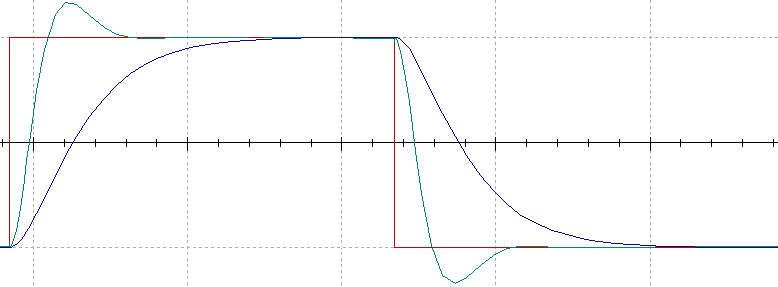
\includegraphics[width=0.5\textwidth]{media/respuesta-sobre-multi}
	 	\caption{Respuesta sistema sobreamortiguado - MULTISIM}
	 	\label{fig:respuesta-sobre-multi}
	 \end{figure}
	 
	 \subsection{\textbf{Muestre las gráficas obtenidas con el Osciloscopio implementado para el caso Subamortiguado y Sobreamortiguado en lazo cerrado.}}
	 
	 \subsubsection{\textbf{Sistema subamortiguado}}
	 Prueba en laboratorio del sistema subamortiguado implementado
	 \begin{figure}[h]
	 	\centering
	 	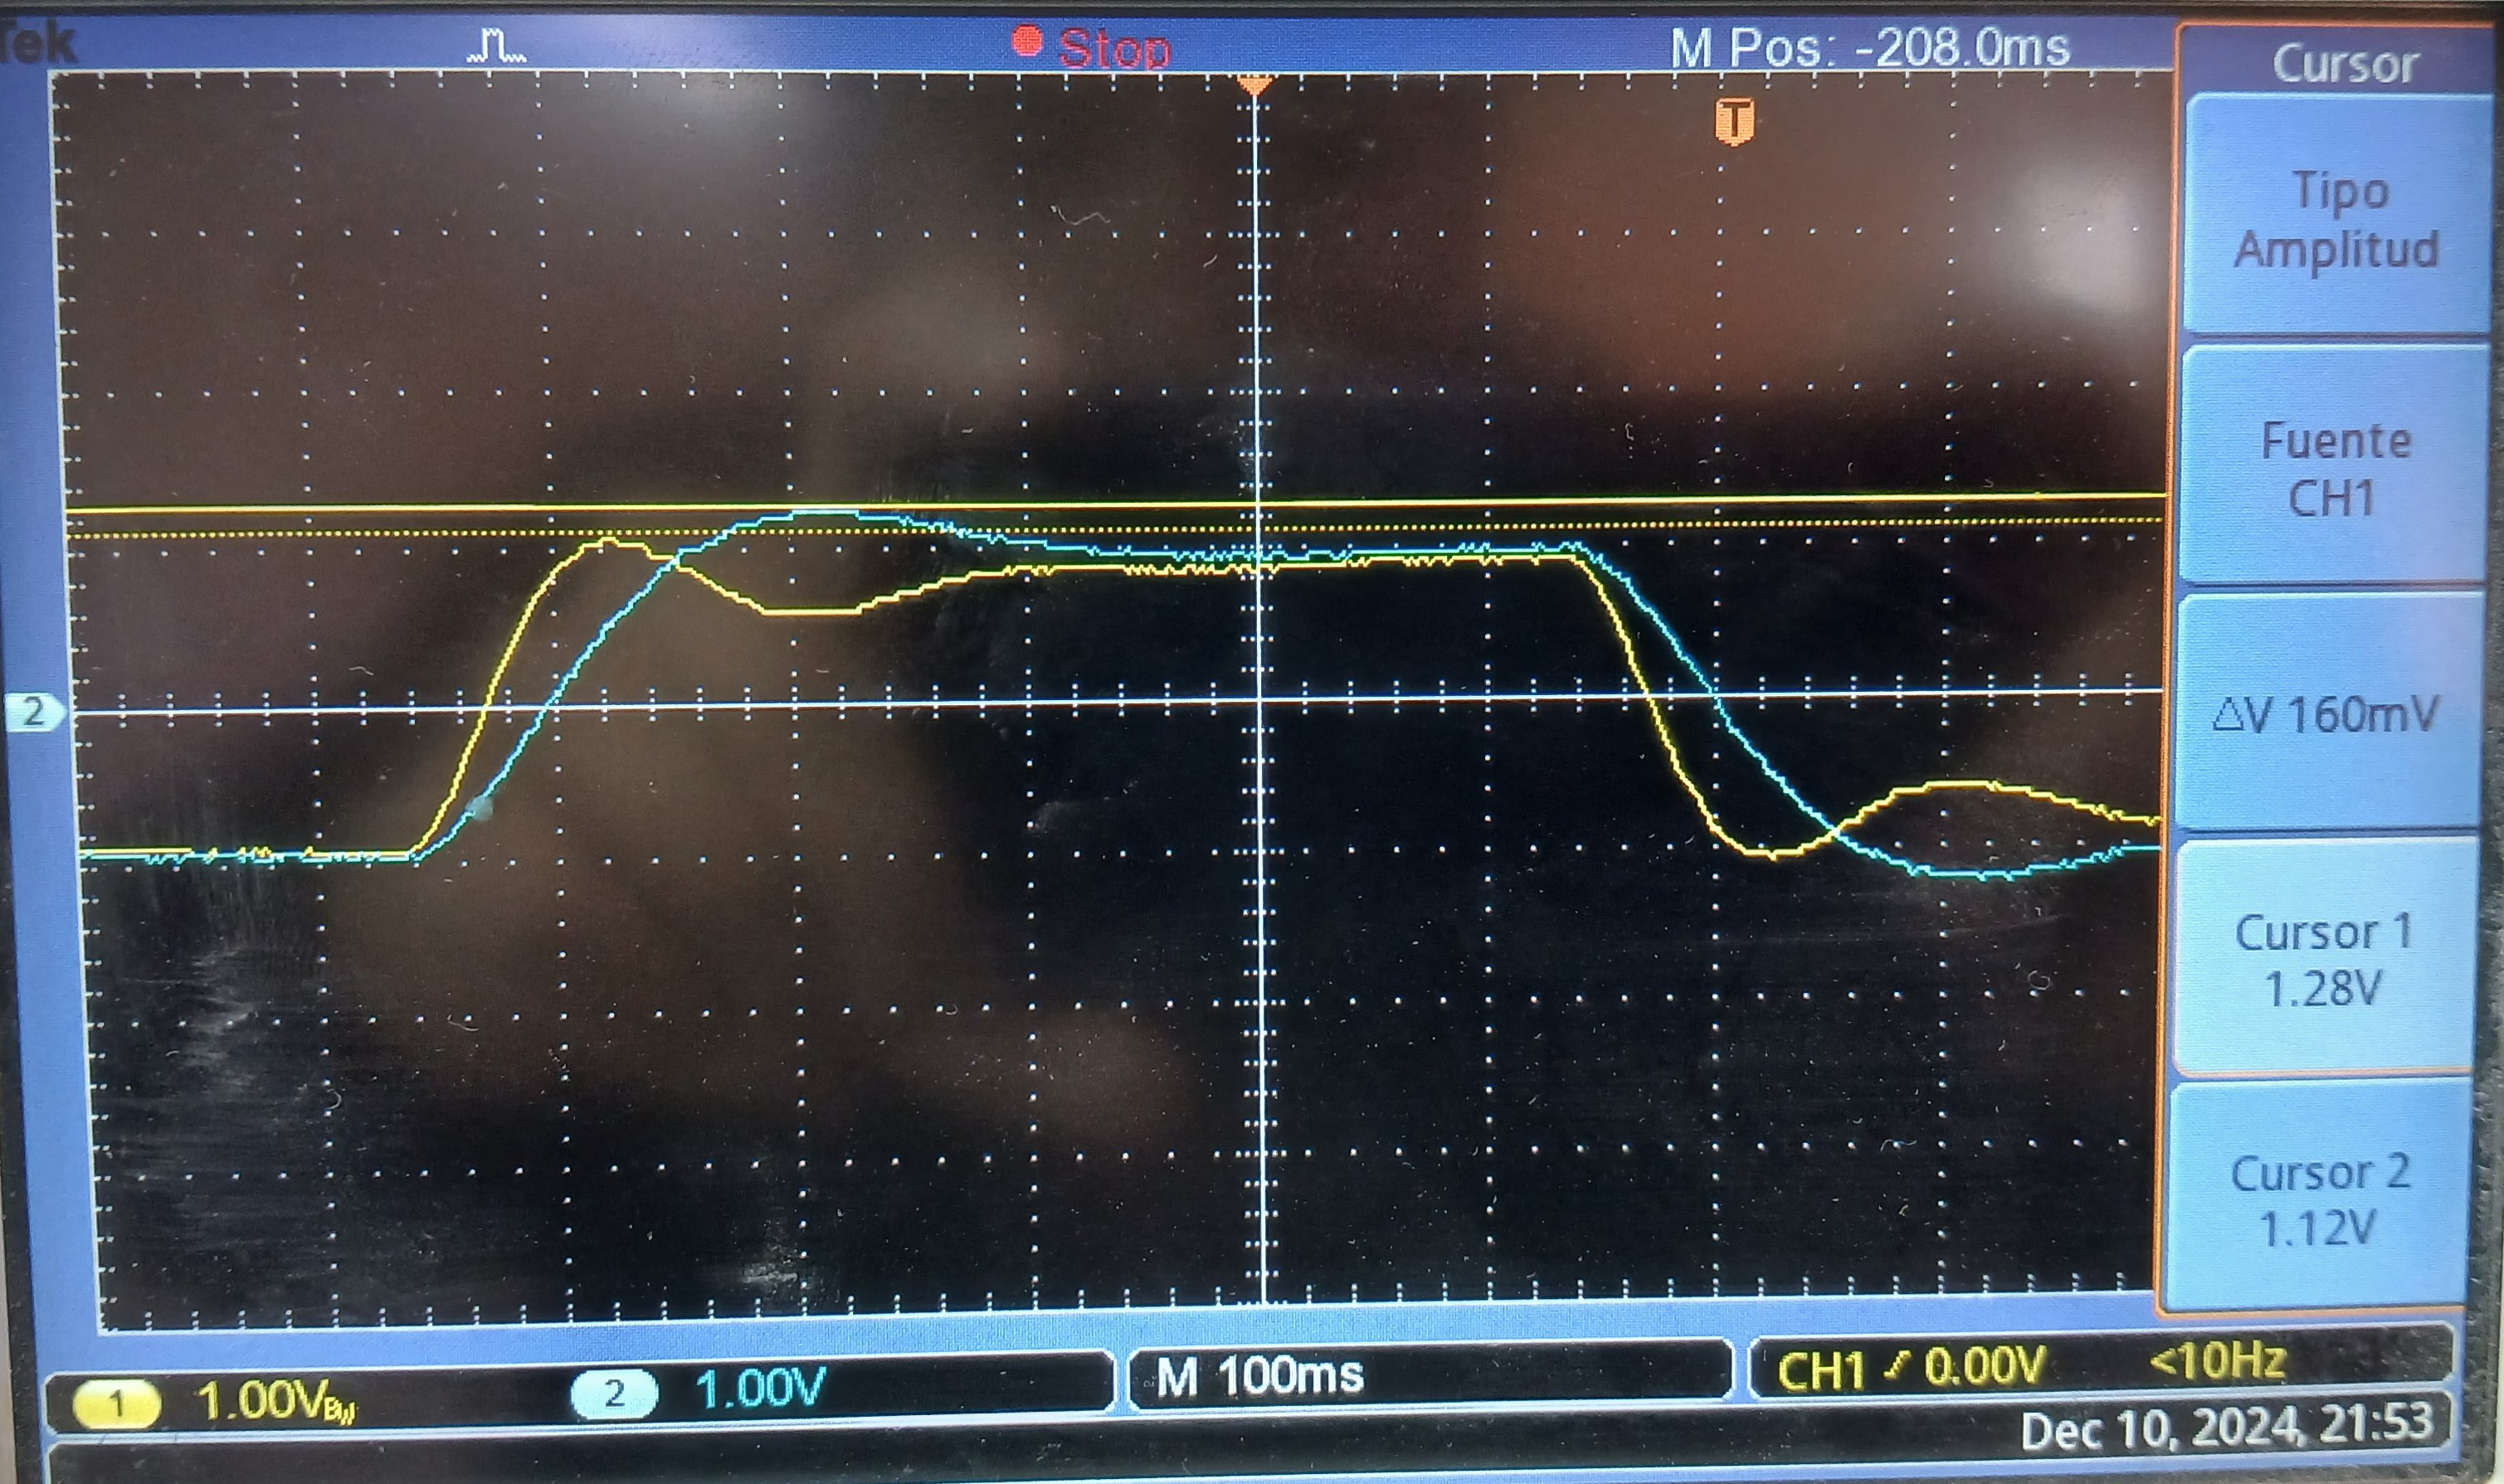
\includegraphics[width=0.5\textwidth]{media/respuesta-sub-implementacion}
	 	\caption{Respuesta del sistema subamortiguado - Implementación}
	 	\label{fig:respuesta-sub-implementacion}
	 \end{figure}
	 
	 En la figura \ref{fig:respuesta-sub-implementacion} se observa la respuesta de un sistema subamortiguado, el cual presenta oscilaciones notables alrededor del valor de referencia antes de estabilizarse, estas oscilaciones disminuyen progresivamente en amplitud con el tiempo debido a la amortiguación, pero la respuesta sigue siendo dinámica y muestra un sobreimpulso antes de converger al valor final.
	 
	 \subsubsection{\textbf{Sistema sobreamortiguado}}
	 Prueba en laboratorio del sistema subamortiguado implementado
	 \begin{figure}[h]
	 	\centering
	 	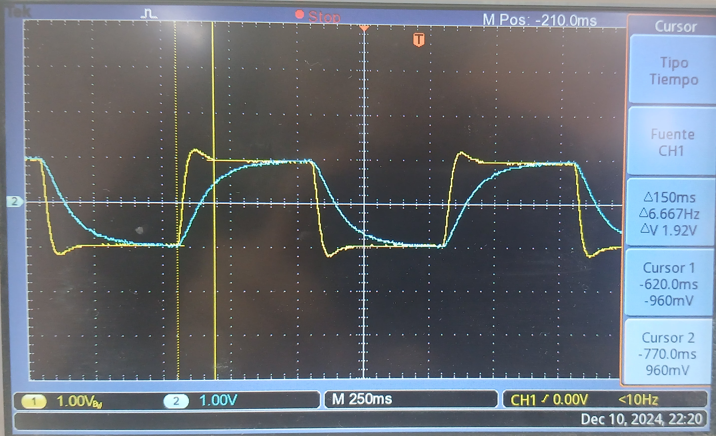
\includegraphics[width=0.5\textwidth]{media/respuesta-sobre-implementacion}
	 	\caption{Respuesta del sistema sistema sobreamortiguado Implementación}
	 	\label{fig:respuesta-sobre-implementacion}
	 \end{figure}
	 
	 En la figura \ref{fig:respuesta-sobre-implementacion} muestra una respuesta mucho más rápida y sin oscilaciones lo cual es característico para este tipo de sistema el cual se aproxima gradualmente al valor de referencia, priorizando la estabilidad sobre la rapidez. La ausencia de oscilaciones evidencia que este tipo de sistema está diseñado para evitar fluctuaciones, aunque a costa de un tiempo de asentamiento un tanto más distanciado.	 
	 
	
	 \subsection{\textbf{Analice el error en estado estacionario en el caso Subamortiguado y Sobreamortiguado en lazo cerrado.}}
	 
	 El error en estado estacionario se refiere al valor de la diferencia entre la señal de entrada deseada y la señal de salida real de un sistema de control, cuando este ha alcanzado un estado estable. Es decir, es el error que persiste en el sistema después de que las transitorias han decaído. Este error es un indicador de la precisión con la que el sistema sigue la señal de referencia.
	 
	 Matemáticamente este se define como 
	 \begin{equation}
	 	K_p = \lim_{s \to 0} G_c G(s)
	 	\label{eq:error-estado-estacionario-limite}
	 \end{equation}
	 Y en la cual $K_p$ es la constante de posición del sistema y la cual se analiza en los sistemas de orden 0 o que no tienen ningún polo en el origen.
	 En análisis del error de estado estacionario además del calculo de la constante de posición es necesario el calculo del mismo error, el cual se realiza mediante \ref{eq:error-estado-estacionario}
	 
	 \begin{equation}
	 	e_{ss} = \frac{1}{1 + K_p}
	 	\label{eq:error-estado-estacionario}
	 \end{equation}
	 
	 \subsubsection{\textbf{Sistema subamortiguado}}
	 \begin{align}
	 	K_p &= \frac{2.5659(10)(25)(325)}{(43.36)(0.1148)(325)} \\
	 	K_p &= 128.86 \\
	 	e_{ss} &= 0.00770
	 \end{align}
	 
	 \subsubsection{\textbf{Sistema sobreamortiguado}}
	 \begin{align}
	 	K_p &= \frac{10.8843(41.98)(16.8)(440.75)}{(117.4)(0.5112)(440.75)} \\
	 	K_p &= 127.9066 \\
	 	e_{ss} &= 0.00775 \\
	 \end{align}
	 Como se puede apreciar para cada el error en estado estacionar es mucho menor al 0.1\% del valor de establecimiento lo cual es un buen indicador debido a que ello indica que el sistema tendrá un establecimiento a pesar de la modificación en la respuesta del sistema al agregar los compensadores.
	 
	 \subsection{\textbf{¿La respuesta hallada en forma teórica es igual o similar al circuito implementado?}}
	 
	 Aunque se puede apreciar diferencias entre cada resultado, estas de forma porcentual no representan un cambio significativo entre las respuestas simuladas e implementados, sin embargo cada destacar que los niveles de voltaje entre las respuestas transitorias y de régimen permanente si se ven alterados por los factores de exactitud en los componentes utilizados, así como el consumo energético y variación en el voltaje de salida qe producen los amplificadores operaciones y el ruido inyectado en la respuesta debido a la interferencia electromagnética de las maquinas electrónicas.
	 
	 \section{conclusiones}
	 La principal diferencia de los sistemas radica en el tiempo de respuesta y las oscilaciones mientras uno es más rápido, presenta oscilaciones, lo que podría ser problemático en sistemas donde la estabilidad inmediata es crítica. Por otro lado, el sistema sobreamortiguado evita estas oscilaciones, pero lo hace sacrificando la rapidez, lo que puede ser menos eficiente en aplicaciones donde se requiere una respuesta ágil.
	 
	\bibliographystyle{IEEEtran}
	\bibliography{biblio}
\end{document}